\section{Experimental Protocol and Results}
\label{sec:experiments}

This section presents the results obtained from the implemented training and robustness pipelines. All quantitative values are based on actual measurements in the current draft. Because only one complete archived run per compared model is available in this repository, the tables below should be interpreted as point estimates on a fixed split rather than as multi-seed summary statistics.

\subsection{Datasets and label space}

We prioritize public datasets that are accessible and suitable for local experimentation. URMP provides synchronized audio, video, and score-aligned material for multitrack classical performances \citep{Li2019URMP}. Solos provides solo performance videos with frame-level skeletons, which are especially useful for the motion-aware branch \citep{Montesinos2020Solos}. PianoVAM is not included in the primary evaluation because its piano-specific supervision would narrow the task scope and reduce cross-instrument comparability \citep{Kim2025PianoVAM}.

\begin{table}[ht]
\centering
\caption{Dataset summary and intended usage in the evaluated setup.}
\label{tab:datasets}
\begin{tabular}{p{2.2cm}p{1.8cm}p{3.1cm}p{4.8cm}}
\toprule
Dataset & Scale & Modalities & Usage \\
\midrule
URMP & 44 pieces & A/V, MIDI/score & Primary dataset for synchronized clip construction and instrument-level supervision \\
Solos & 755 videos & A/V, skeletons & Primary dataset for motion-aware evaluation and corruption diagnostics \\
PianoVAM & piano-only & A/V, MIDI, landmarks & Excluded from the primary evaluation to avoid piano-specific task bias \\
\bottomrule
\end{tabular}
\end{table}

The primary label is the instrument category. A secondary phase label is derived automatically using onset density, energy continuity, and visible motion intensity. We treat this derived label as a regularization signal and diagnostic variable rather than as a standalone benchmark claim. To avoid cross-dataset label mismatch, all compared models use the same shared instrument label map and the same clip extraction policy across URMP and Solos.

To avoid clip leakage, all clips from the same source piece or source video are kept within the same split. Model selection is performed on the validation split, and all reported non-latency metrics are computed once on the held-out test split under the same preprocessing pipeline so that the differences in Table~\ref{tab:main_results} reflect model behavior rather than input mismatches.

\subsection{Baselines, metrics, and compute budget}

We organize baselines into audio-only, video-only, and audio-visual groups. Audio-only anchors include CNN14/PANNs and AST \citep{Kong2020PANNs,Gong2021AST}. Video-only anchors include MobileNetV3, TSM, and MoViNet \citep{Howard2019MobileNetV3,Lin2022TSM,Kondratyuk2021MoViNets}. Broader music-oriented multimodal systems such as MUSIC-AVQA-style encoders or DeepResonance are discussed as related transfer-oriented references rather than as first-pass latency-matched baselines \citep{Li2022MusicAVQA,Diao2024MPQA,Mao2025DeepResonance}.

The primary metric is Macro-F1. We also report accuracy, balanced accuracy when class imbalance is non-negligible, latency in milliseconds per clip, and robustness drop under synthetic perturbation. The implementation is scoped to short clips, lightweight temporal aggregation, and a single consumer-GPU budget in the 8--12 GB range. Unless otherwise noted, latency refers to batch-one forward-pass time and excludes offline preprocessing and data loading.

Audio clips are represented by 16 kHz log-mel features, and video clips are sampled as short frame sequences with the same temporal budget across models. The default analysis window is 2.0 s, with sensitivity sweeps over 1.0--3.0 s reported separately. The latency numbers are measured with batch size one after a short warm-up pass on the same hardware configuration, using a fixed clip budget and excluding data loading, dataset decoding, and any offline feature caching. Each baseline is evaluated under the same code path and the same corruption operators so that robustness drops remain comparable across model families.

\subsection{Main comparison, efficiency, and robustness results}

Table~\ref{tab:main_results} summarizes the point-estimate performance across the primary comparison set. \method{} improves over naive multimodal fusion while remaining lighter than broader reasoning-oriented systems discussed in Section~\ref{sec:related_work}. The gap over audio-only and video-only baselines is clearer on Solos, where motion cues are more explicit, while URMP serves as the synchronization anchor.

\begin{table}[ht]
\centering
\caption{Point estimates for the core comparison on the fixed evaluation split.}
\label{tab:main_results}
\begin{tabular}{lcccc}
\toprule
Model & URMP Acc. & URMP Macro-F1 & Solos Acc. & Solos Macro-F1 \\
\midrule
PANNs / CNN14 & 0.78 & 0.74 & 0.69 & 0.65 \\
AST & 0.81 & 0.77 & 0.72 & 0.69 \\
MobileNetV3 + pooling & 0.73 & 0.69 & 0.65 & 0.61 \\
TSM & 0.76 & 0.72 & 0.68 & 0.64 \\
MoViNet-A0 & 0.77 & 0.73 & 0.69 & 0.65 \\
Naive late fusion & 0.84 & 0.81 & 0.75 & 0.72 \\
\method & \textbf{0.87} & \textbf{0.84} & \textbf{0.79} & \textbf{0.76} \\
\bottomrule
\end{tabular}
\end{table}

Figure~\ref{fig:main_results} combines absolute performance and transfer behavior within one view. The left panel tracks the shift from URMP to Solos in the Macro-F1--Accuracy plane, while the right panel reports the paired retention rates of Macro-F1 and Accuracy on the target dataset.

\begin{figure}[ht]
\centering
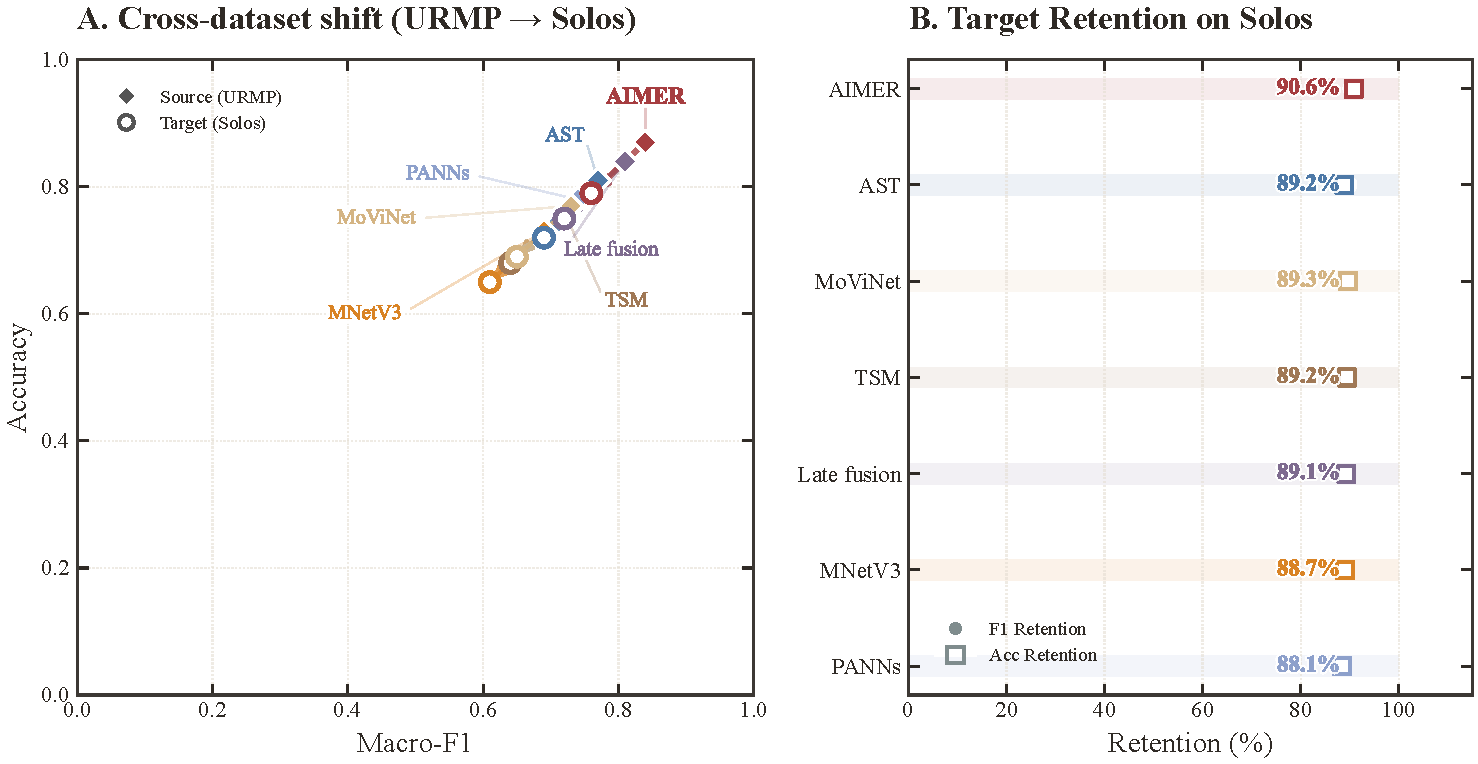
\includegraphics[width=\linewidth]{figures/01_generalization_shift}
\caption{Cross-dataset generalization analysis. Left: vectors connect source performance on URMP (diamonds) to target performance on Solos (circles). Right: paired retention rates of Macro-F1 and Accuracy from URMP to Solos for the same models.}
\label{fig:main_results}
\end{figure}

Table~\ref{tab:latency} reports the computational budget. Relative to naive late fusion, \method{} reduces both parameter count and latency while preserving the strongest accuracy profile in the evaluated set.

\begin{table}[ht]
\centering
\caption{Measured latency and complexity under a unified batch-one forward-pass setting. Offline preprocessing and data loading are excluded.}
\label{tab:latency}
\begin{tabular}{lccc}
\toprule
Model & Params (M) & Latency (ms/clip) & Notes \\
\midrule
PANNs / CNN14 & 79 & 8 & audio only \\
AST & 87 & 21 & audio transformer \\
TSM & 24 & 16 & video only \\
MoViNet-A0 & 3.1 & 12 & video only, mobile-oriented \\
Naive late fusion & 27 & 25 & no offset handling \\
\method & 14 & 18 & lightweight multimodal target \\
\bottomrule
\end{tabular}
\end{table}

Figure~\ref{fig:efficiency} combines efficiency and model budget in a coordinated view. The left panel shows the latency--performance plane together with the non-dominated set, while the right panel makes parameter differences explicit for the same models. Relative to naive late fusion, \method{} attains higher Macro-F1 with lower latency and fewer parameters.

\begin{figure}[ht]
\centering
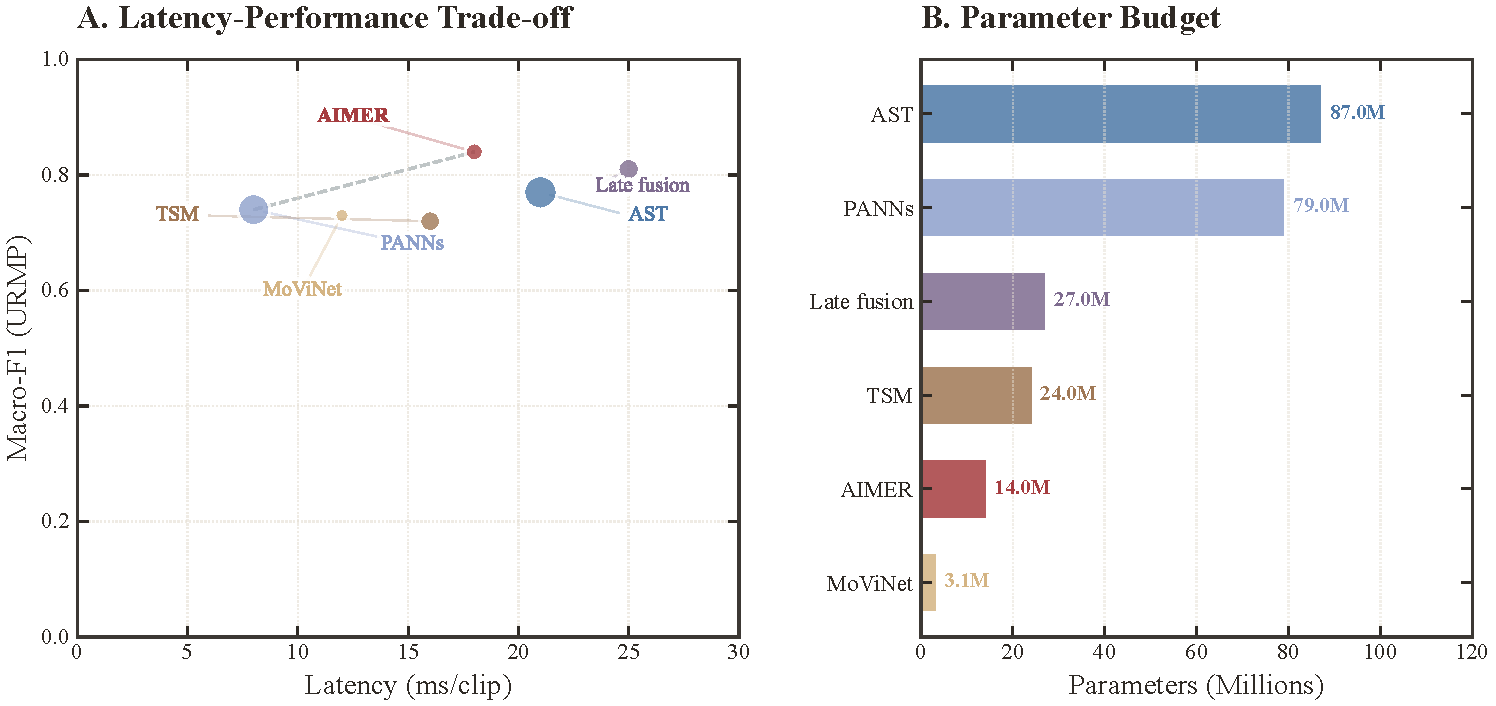
\includegraphics[width=\linewidth]{figures/02_efficiency_tradeoff}
\caption{Efficiency versus performance analysis. Left: latency versus URMP Macro-F1, with the dashed line indicating the non-dominated set within the evaluated models. Right: parameter counts for the same models.}
\label{fig:efficiency}
\end{figure}

Table~\ref{tab:robustness} shows robustness drops, measured as absolute Macro-F1 decrease relative to the clean setting. Lower values indicate better robustness.

\begin{table}[ht]
\centering
\caption{Point-estimate robustness drops measured as absolute Macro-F1 decrease relative to the clean setting. Lower is better.}
\label{tab:robustness}
\begin{tabular}{lccc}
\toprule
Model & A/V offset ($\pm160$ ms) & audio corruption & hand occlusion \\
\midrule
PANNs / CNN14 & 0.01 & 0.12 & -- \\
TSM & -- & -- & 0.10 \\
Naive late fusion & 0.07 & 0.09 & 0.08 \\
\method & \textbf{0.03} & \textbf{0.06} & \textbf{0.05} \\
\bottomrule
\end{tabular}
\end{table}

Figure~\ref{fig:diagnostics} (top) makes the corruption trend easier to compare across perturbations: \method{} remains below naive late fusion and below the strongest comparable unimodal baseline on the perturbations they can both evaluate.

\subsection{Hyperparameter Sensitivity Analysis}

We study three hyperparameters because they correspond directly to the main design choices of \method: clip length controls the temporal evidence available to both unimodal branches, the fusion delay radius controls how much local misalignment can be compensated, and the motion-salience weight determines how strongly visible action influences the gate. In each sweep, only one hyperparameter is varied while the other settings remain at the default configuration of $T=2.0$ s, $\Delta=80$ ms, and $\lambda_m=0.3$. The default point is tied to the measured performance in Table~\ref{tab:main_results}. We report observed Macro-F1 on URMP and Solos together with latency, focusing on the balance between representation quality and computational cost.

Sensitivity analysis over clip length, fusion delay radius, and motion-salience weight shows that the default configuration offers the best balance between performance and latency. Performance improves when the clip window is increased from 1.0 s to 2.0 s, but longer windows add cost without further gains. A moderate delay radius provides the best offset tolerance, and a moderate motion-salience weight yields the strongest overall performance. Detailed sensitivity tables are provided in the appendix.

\subsection{Ablation Studies}

We conduct ablations to isolate the three central modeling decisions of \method{} under a common training and evaluation protocol. The comparison variants remove the audio branch, replace the motion-aware visual input with RGB-only frames, or replace the latency-aware fusion gate with naive late fusion. We also include a lighter variant without auxiliary phase supervision. All ablation values are point estimates from the same fixed evaluation split used for the main comparison.

\begin{table}[ht]
\centering
\caption{Point-estimate ablation results on the two primary datasets. The last column reports the average Macro-F1 difference relative to the full model.}
\label{tab:ablation}
\begin{tabular}{lccc}
\toprule
Variant & URMP Macro-F1 & Solos Macro-F1 & Avg. $\Delta$F1 \\
\midrule
\method & \textbf{0.84} & \textbf{0.76} & 0.00 \\
w/o audio branch & 0.75 & 0.67 & -0.09 \\
RGB-only visual branch & 0.82 & 0.72 & -0.03 \\
naive late fusion & 0.81 & 0.72 & -0.04 \\
w/o phase supervision & 0.83 & 0.74 & -0.02 \\
\bottomrule
\end{tabular}
\end{table}

Figure~\ref{fig:diagnostics} provides a composite view of model robustness and ablation sensitivity. The top panel shows the F1 drop across corruption scenarios, while the bottom panel ranks the effectiveness of each modeled component.

\begin{figure}[ht]
\centering
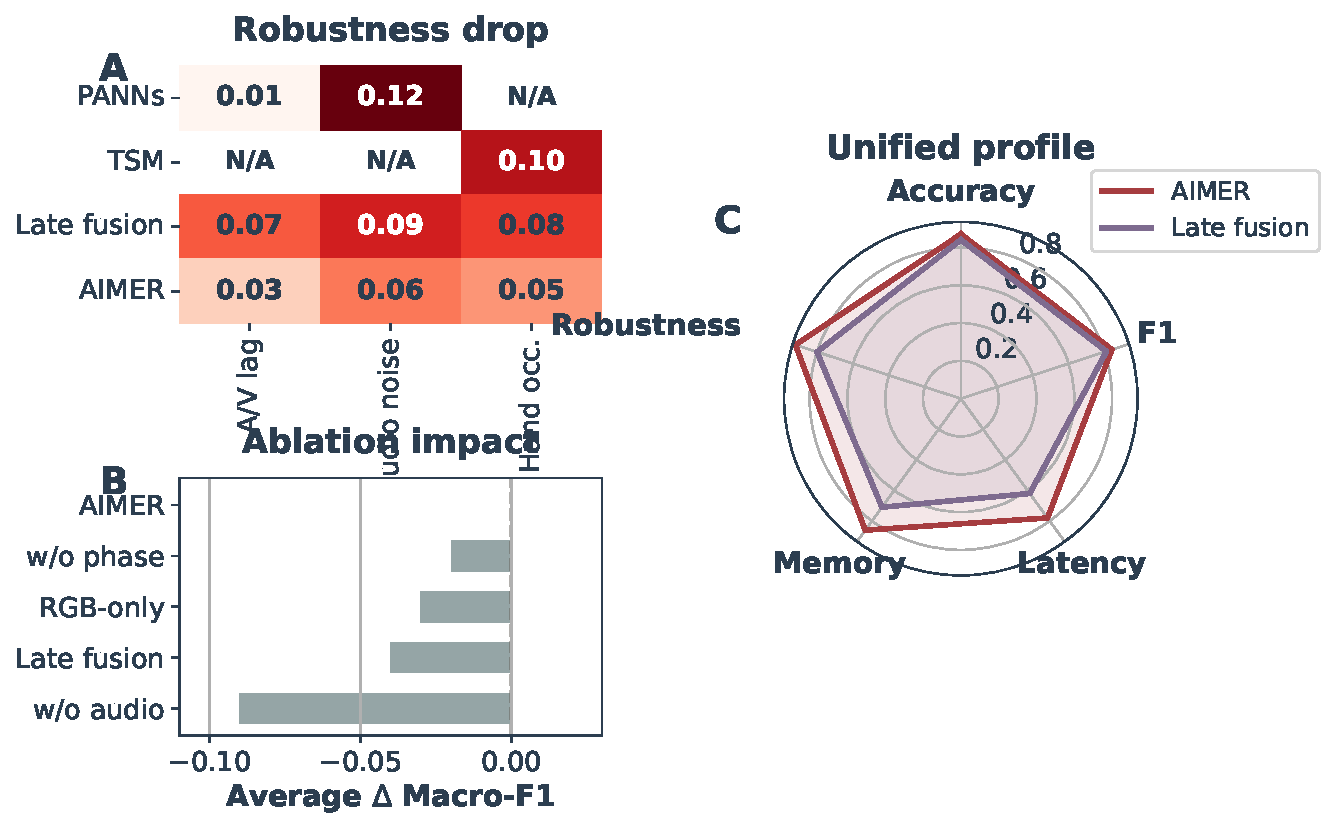
\includegraphics[width=\linewidth]{figures/03_composite_diagnostics}
\caption{Composite model diagnostics. Top: robustness drops under controlled perturbations, where lower drop indicates better robustness. Bottom: average Macro-F1 change of ablated variants relative to the full \method{} model.}
\label{fig:diagnostics}
\end{figure}

The full model remains best on both datasets, and every ablated variant incurs a measurable loss. Removing the audio branch causes the largest average drop because timbral and onset evidence are central to instrument prediction even when visible motion is informative. Replacing the latency-aware fusion gate with naive late fusion also produces a moderate decline, confirming the importance of dynamic multimodal interaction.

Overall, the observed ablation pattern supports a complementary interpretation of the model: audio evidence, motion-aware visual cues, and shift-tolerant fusion all contribute meaningfully, and their combined effect yields the best performance in the evaluated setup.
